\chapter{ Область устойчивости}
\label{ch:chap2}

\ExplSyntaxOn
\clist_new:N \l_feq_vector_clist
\NewDocumentCommand{\feqvector}{O{\\}mO{b}}{
  \clist_set:Nn \l_feq_vector_clist {#2} % Set the list
  \begin{#3matrix}
  \clist_use:Nn \l_feq_vector_clist {#1} % show it with separator from #1 (\\)
  \end{#3matrix}
}
\ExplSyntaxOff


\definecolor{codegreen}{rgb}{0,0.6,0}
\definecolor{codegray}{rgb}{0.5,0.5,0.5}
\definecolor{codepurple}{rgb}{0.58,0,0.82}
\definecolor{backcolour}{rgb}{0.95,0.95,0.92}

\lstdefinestyle{mystyle}{
    backgroundcolor=\color{backcolour},   
    commentstyle=\color{codegreen},
    keywordstyle=\color{magenta},
    numberstyle=\tiny\color{codegray},
    stringstyle=\color{codepurple},
    basicstyle=\ttfamily\footnotesize,
    breakatwhitespace=false,         
    breaklines=true,                 
    captionpos=b,                    
    keepspaces=true,                 
    numbers=left,                    
    numbersep=5pt,                  
    showspaces=false,                
    showstringspaces=false,
    showtabs=false,                  
    tabsize=2
}
\lstset{style=mystyle}

\section{Изучаем пространство параметров}
В этом задании мы будем работать со следующей структурной схемой:
\begin{figure}[ht]
  \centering
  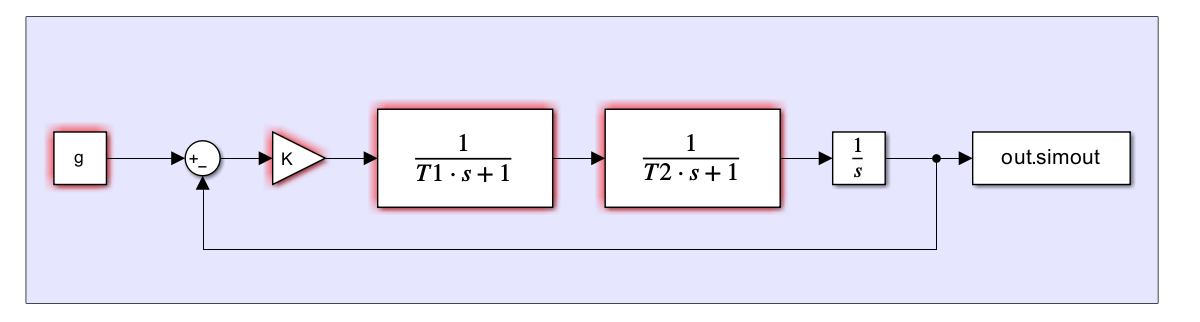
\includegraphics[width=0.8\textwidth]{scheme_system2.png}
\caption{Структурная схема - система 3-го порядка}
\end{figure}
Объеденим две передаточные функции из схемы выше в одну:
$$
W_{12}(s) = \frac{1}{(T_1s+1)(T_2s+1)}
$$
Вспомним как выглядела передаточная функция из первого задания, которую можно упростить, заменив уравнение решениями через лямбды, которые давали нам для эксперементов, так как по заданию мы смотрим на первый эксперемент, то упростим при помощи $\lambda_1,\lambda_2$:
$$
W_{3}(s) = \frac{1}{s^2 + a_1s + a_0} =\frac{1}{(s-\lambda_1)(s-\lambda_2)}
$$
Приравняем передаточные функции, тогда сможем найти $T_1, T_2$, при которых полюса(читать как "знаменатель") соответствующих передаточных функций совпадут с первым набором корней:
$$
\begin{aligned}
  \frac{1}{(s-\lambda_1)(s-\lambda_2)} = \frac{1}{(T_1s+1)(T_2s+1)} = \dots \\
  \begin{cases}
      s = \lambda_1\\
      s = \lambda_2 \\
      T_1s + 1 = 0 \\
      T_2s + 1 = 0,
   \end{cases} \\
   \begin{cases}
      T_1\lambda_1 + 1 = 0 \\
      T_2\lambda_2 + 1 = 0,
 \end{cases} \\
 \begin{cases}
    T_1 = -\frac{1}{\lambda_1} = -\frac{1}{-1} = 1\\
    T_2 = -\frac{1}{\lambda_1} = -\frac{1}{-1.5} = \frac{2}{3} 
  \end{cases}
\end{aligned}
$$

Теперь зафиксируем $T_2 = \frac{2}{3}$ и зададимся вопросом устойчивости в пространстве параметров $K,T_1$ в смысле критерия Гурвица. 

Для этого восстановим дифференциальное уравнение из структурной схемы задания, для начала зафиксируем, что $g$ - входной сигнал, а $y$ - выходной, $s$ - оператор дифференцирования:
$$
\begin{aligned}
  y = \frac{1}{s}\bigg(  \frac{1}{(T_1s+1)(T_2s+1)}\bigg( K(g-y) \bigg) \bigg) \\
  y = \frac{K(g-y)}{s(T_1s+1)(T_2s+1)} \\
  y = \frac{K(g-y)}{s(T_1s+1)(T_2s+1)} \\
  y = \frac{K(g-y)}{T_1T_2s^3+(T_1+T_2)s^2 + s} \\
\end{aligned}
$$
Теперь раскроем передаточную функцию, также вспомним, что мы работаем со свободным движением, поэтому $g=0$ будет:
$$
\begin{aligned}
  K(g-y) = T_1T_2s^3[y]+(T_1+T_2)s^2[y] + s[y] \\
  g = y + \frac{1}{K}\bigg(  T_1T_2s^3[y]+(T_1+T_2)s^2[y] + s[y] \bigg) \\
  y + \frac{1}{K}\bigg(  T_1T_2s^3[y]+(T_1+T_2)s^2[y] + s[y] \bigg) = 0 \bigg|:\frac{K}{T_1T_2} \\
  s^3[y]+ \frac{T_1+T_2}{T_1T_2}s^2[y] + \frac{1}{T_1T_2}s[y] + \frac{K}{T_1T_2}y = 0
\end{aligned}
$$
Тогда получим следующие коэффициенты системы:
$$
a_2 = \frac{T_1+T_2}{T_1T_2}, \tab a_1 =\frac{1}{T_1T_2}, \tab a_0= \frac{K}{T_1T_2};
$$
Критерий Гурвица для систем третьего порядка формулируется следующим образом:
$$
\begin{cases}
  a_0,a_1,a_2 > 0 \\
  a_2a_1>a_0
\end{cases}
$$
В нашем случае слагаемые системы будут выглядеть так(читать горизонтально):
$$
\begin{cases}
  \frac{T_1+T_2}{T_1T_2}>0, \tab \frac{1}{T_1T_2}>0, \tab \frac{K}{T_1T_2}>0 \\
  \frac{T_1+T_2}{(T_1T_2)^2}>\frac{K}{T_1T_2}
\end{cases}
$$ 
Немного упростим эту громоздкую систему, сразу подставив $T_2 = \frac{2}{3}$:
$$
\begin{cases}
  T_1 > 0\\
  K > 0\\
  \frac{T_1+\frac{2}{3}}{\frac{2}{3}T_1}>K
\end{cases}
$$ 
Удобно мы сможем построить эту систему в программе \textit{Desmos}, область устойчивости обозначена синим цветом, а граница - красным:
\begin{figure}[ht]
  \centering
  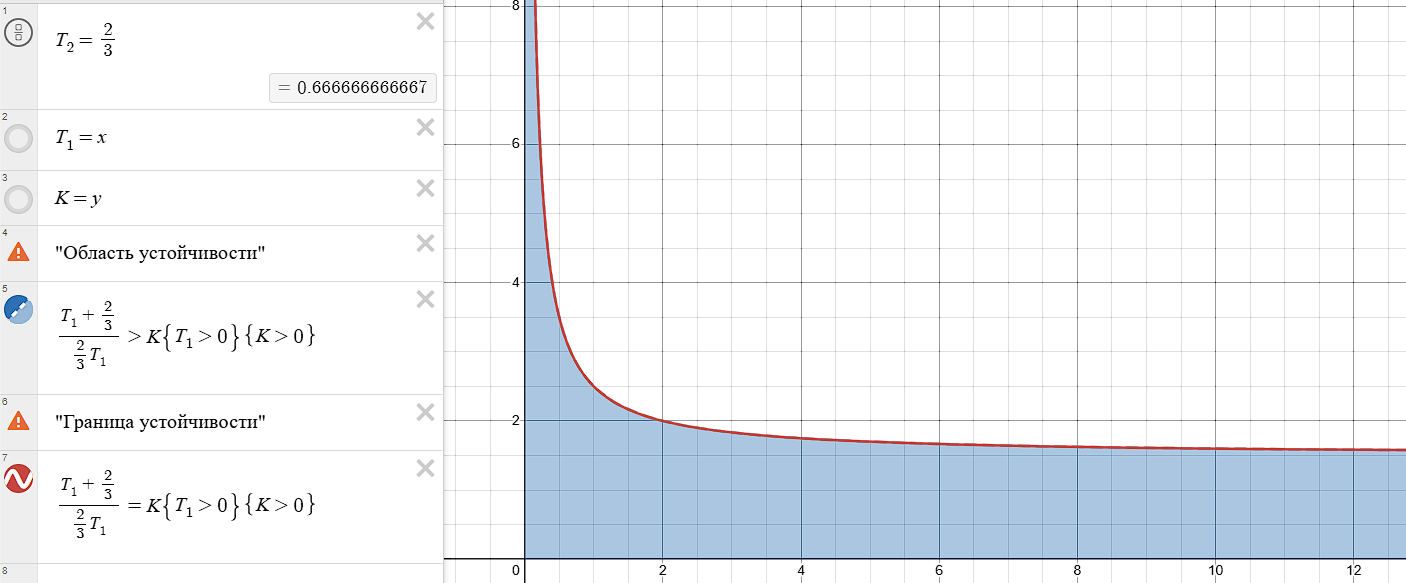
\includegraphics[width=0.8\textwidth]{plot_K(T1).png}
\caption{Пространство параметров $K(T_1)$ - область и граница устойчивости}
\end{figure}

Далее по аналогии аналитически определим границу и область устойчивости в пространстве параметров $K(T_2)$, то есть уже при фиксированном $T_1 = 1$. Моделирование осуществляем при $u(t)=1$
Теперь система будет выглядеть следующим образом:
$$
\begin{cases}
  T_2 > 0\\
  K > 0\\
  \frac{T_2+ 1}{T_2}>K
\end{cases}
$$ 
Тогда пространство параметров будет выглядеть вот так, область устойчивости обозначена синим цветом, а граница - красным:
\begin{figure}[ht]
  \centering
  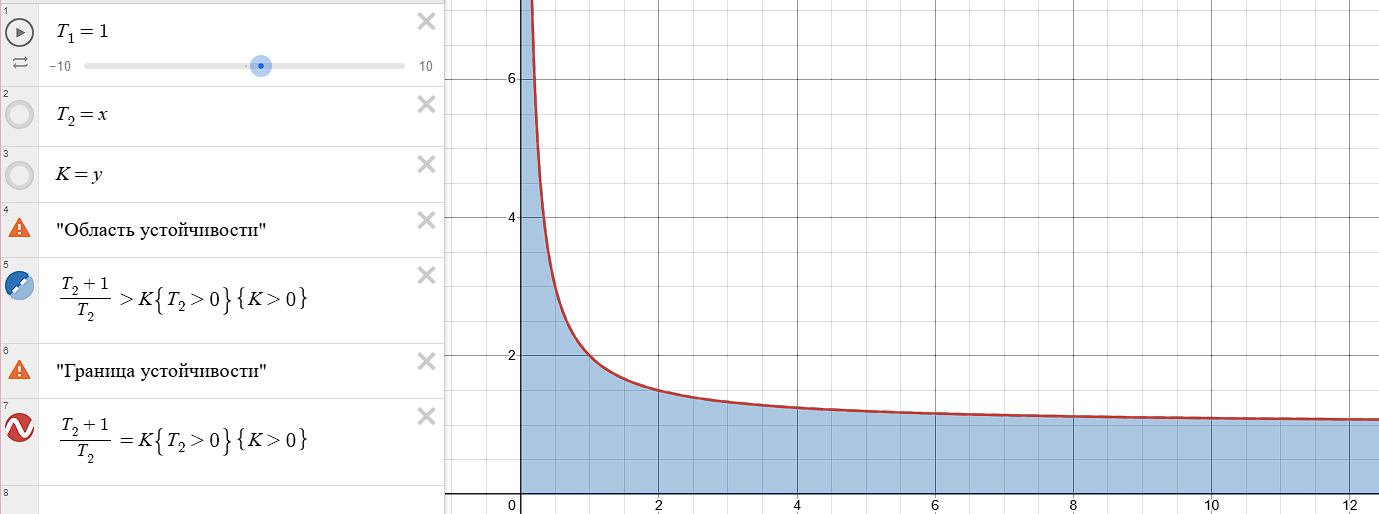
\includegraphics[width=0.6\textwidth]{plot_K(T2).png}
\caption{Пространство параметров $K(T_2)$ - область и граница устойчивости}
\end{figure}

\section{Симулируем устойчивости}
Зададимся тремя наборами параметров $K, T_1, T_2$, которые соответствуют трём усточивостям.
При выборе коэффициентов я опирался на пространства параметров, полученные выше\dots
\subsection{Асимптотически устойчивая система}
$$
K=0.5,\tab T_1=1,\tab T_2=5
$$
\begin{figure}[ht]
  \centering
  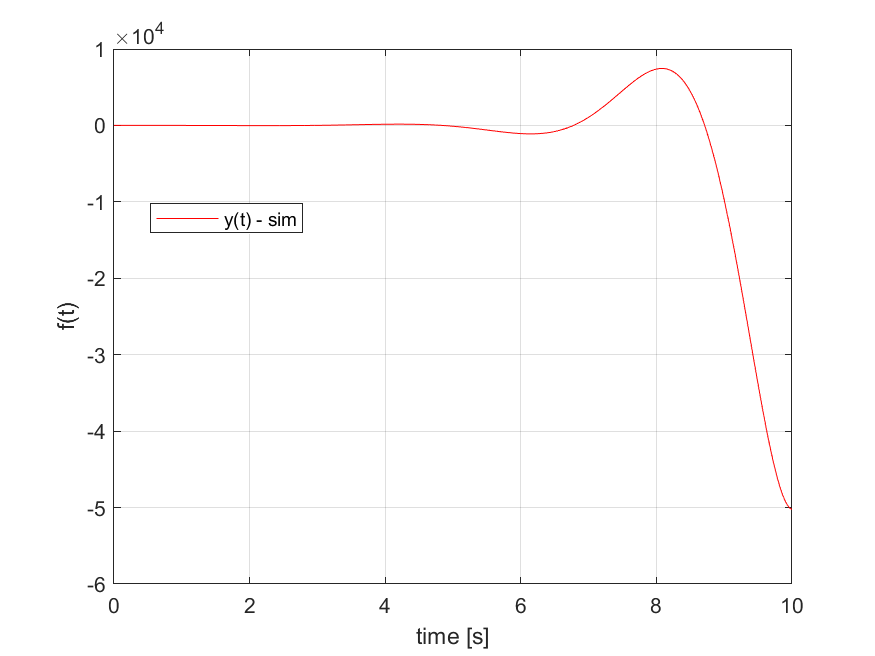
\includegraphics[width=0.9\textwidth]{output_task2_exp1.png}
\caption{Асимптотически устойчивая система}
\end{figure}
Система \textbf{асимпотитечки устойчива}, так как сходится к "нулю".
\newpage
\subsection{Гранично устойчивая система}
$$
K=9,\tab T_1=1,\tab T_2=\frac{1}{8}
$$
\begin{figure}[ht]
  \centering
  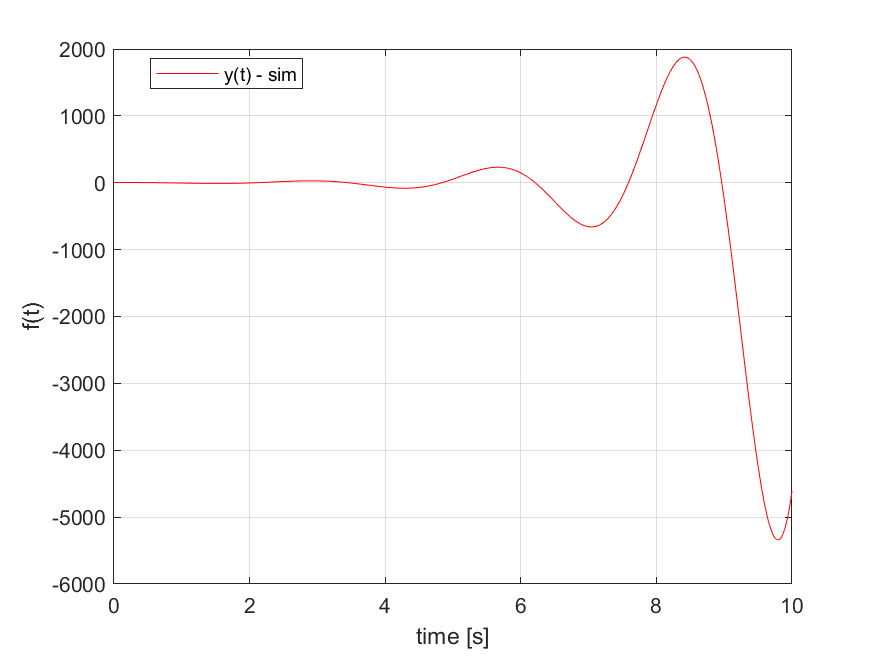
\includegraphics[width=0.9\textwidth]{output_task2_exp2.png}
\caption{Гранично устойчивая система}
\end{figure}
Система соответствует \textbf{устойчивости по Ляпунову}, так как ограничена сверху и снизу.
\newpage
\subsection{Неустойчивая система}
$$
K=4,\tab T_1=4,\tab T_2= \frac{2}{3}
$$
\begin{figure}[ht]
  \centering
  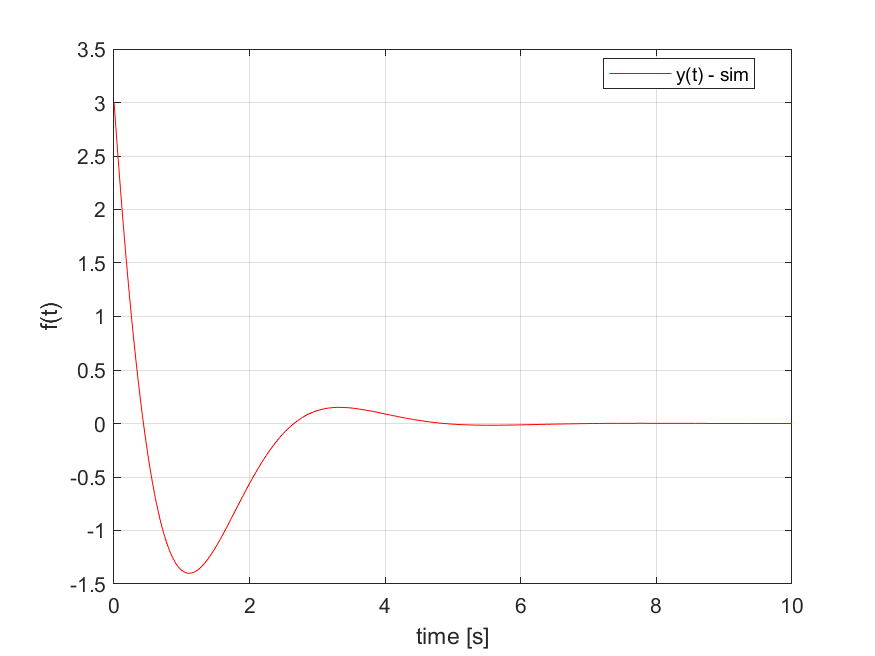
\includegraphics[width=0.9\textwidth]{output_task2_exp3.png}
\caption{Неустойчивая система}
\end{figure}
Система \textbf{неустойчива}, так как улетает в бесконечность.

\section{Выводы}
В итоге, мы изучили систему третьего порядка посредством осмотра её пространства параметров при одном фиксированном значении. Это дало нам понимания границы и области устойчивости системы, которые мы можем использовать при более сложном анализе. 
Но в нашем случае мы воспользовались этими портретами, чтобы быстро определить три наборы коэффициентов, при котором мы показали три типа устойчивости - асимптотическую, граничную, и неустойчивость.
% \begin{figure}[!ht]
% 	\centering
% \hspace*{\fill}%
% 	\begin{subfigure}[b]{0.49\textwidth}
%         \centering
% 		\includegraphics[width=1\textwidth]{2_18.png}
% 	\end{subfigure}
% \hfill
% 	\begin{subfigure}[b]{0.49\textwidth}
%         \centering
% 		\includegraphics[width=1\textwidth]{2_19.png}
% 	\end{subfigure}
%     \caption{Функция и её сэмплированный вариант}
% \end{figure}



\endinput